
\chapter{Hidden variables for semiclassical models with state-dependent forces}

Hidden variable theories [CITE, CITE] are interpretations of quantum mechanics which posit that there are definite states underlying quantum wavefunctions, such that quantum indeterminacy is an illusion---an emergent phenomenon rather than a fundamental fact. The Bell inequality [CITE] proves that any such theory must be \emph{nonlocal} in order to explain all the predictions of quantum mechanics, and perhaps in light of this, most physicists surveyed [CITE] do not believe that hidden variables underlie physical reality.

However, by framing quantum systems in classical terms, hidden variable theories can provide an excellent computational tool for \emph{approximate} models of quantum systems, when it is reasonable to approximate some degrees of freedom as classical, yet other degrees of freedom need to be modelled quantum mechanically. Just as hidden variable theories have framed the quantum world in terms that are agreeable to the classical view of the world in the minds of some interpreters of quantum mechanics, so can they bridge the gap between a \emph{simulated} quantum world and a \emph{simulated} classical world coexisting in the same computer simulation.

In this chapter I describe what I call the `hidden variables semiclassical' (\textsc{hvsc}) method: a method of combining quantum simulations with classical simulations, with hidden variables bridging the gap between the classical and quantum degrees of freedom. In this introduction I describe existing semiclassical methods, the manner in which their quantum and classical parts are typically coupled based on expectation values (which I'm calling the `Ehrenfest method'), and in which regimes this inaccurate---namely the Stern--Gerlach experiment and similar situations in which considerable entanglement between motional and internal degrees of freedom develop.

In [SECREF THE NEXT SECTION] I give the technical definition of a hidden variable theory, and motivate the use of such a theory for coupling quantum and classical degrees of freedom in such a way that the a semiclassical model can be made to agree more closely than the Ehrenfest method with the underlying fully quantum model it is approximating, and ultimately, with experiment.

In section [SECREF THE SECTION AFTER THAT] I then go into the implications of welcoming a hidden variable into a semiclassical model, including additional required assumptions and approximations, and I derive the equations of motion for the model as a whole. Then in section [SECREF] I discuss the method further including its limitations.

Throughout this chapter, I make comparison between the \textsc{hvsc} and Ehrenfest methods. The two methods share most of the same flaws, save for \textsc{hvsc}'s ability to reproduce the Stern--Gerlach experiment. As such \textsc{hvsc} is an incremental improvement on the Ehrenfest method that solves this one specific problem. My method has a number of crude approximations---namely that wavepackets have a fixed size and that the decoherence of the atom's internal state is Markovian---and the wavepacket size and decoherence rate are estimated using approximate formulae. While crude, this is nonetheless an improvement over the Ehrenfest method's implicit assumption that decoherence does not occur at all (in which case the wavepacket size does not matter, as I will show), which is considerably less correct than even the crudest calculation of a Markovian decoherence rate. The \textsc{hvsc} method forces these assumptions to be made explicit, and serves as a minimal improvement to the Ehrenfest method, taking into account the simplest kind of decoherence only. Further improvements to the method are likely possible, but would be computationally more intensive to implement and unlikely to be worth it given the typical accuracy demanded of semiclassical simulations.


\subsection{Semiclassical models}

A semiclassical model is any model in which some degrees of freedom are treated quantum mechanically, and others classically. The most common combination is that of treating an atom's internal electronic state quantum mechanically and its motional degree of freedom classically. This is useful whenever the quantum effects of the atom's motion are not of interest, for example if temperatures are high and thus atomic wavelengths are short---such that quantum effects simply aren't visible in the motion of the particles and so they can accurately be modelled as classical billiard balls. The energy gaps between different electronic states are so large however that only at very high temperatures (at which atoms ionise anyway) do they start to appear as a continuum compared to thermal energy scales, and the interaction of different spin states of the atom with different optical and magnetic fields does not make them appear as classical continua either. Thus, quantum effects can be ignored for centre of mass motion of the atom, but not for the relative motion of its electrons with respect to the nucleus, or for the nuclear and electronic spin degrees of freedom.

In this regime, atoms are often modelled semiclassically, with these internal degrees of freedom modelled using a state vector $\ket\chi$ evolving according to a Hamiltonian $\hat H$ via the Schr\"odinger equation, and the centre of mass motion modelled as a position $\vec r$ and velocity $\vec v$ evolving according to Newton's second law (\figref{fig:semiclassical}).

\begin{figure}[t]
    \centerfloat
    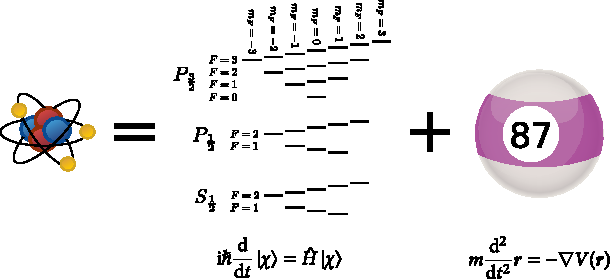
\includegraphics[width=0.75\textwidth]{figures/hidden_variables/semiclassical.pdf}
    \caption{Artist's depiction of a semiclassical atom.}
    \label{fig:semiclassical}
\end{figure}

Once one has defined a potential function $V(\vec r)$ and a Hamiltonian (also possibly varying with space) $\hat H(\vec r)$, and other possible additions\footnote{Such using a Monte-Carlo wavefunction method [CITE, SECREF?] to model the effect of spontaneous emission on $\ket\chi$, and modifying $\vec v$ instantaneously by a random-direction recoil velocity upon each photon emission}, ones job is done and the rest can be left to numerical differential equation solvers to evolve some concrete vector representation $\vec\chi$ of $\ket\chi$ as well as the state variables $\vec r$ and $\vec v$ for motional degree of freedom in time according to the coupled differential equations
\begin{align}\label{eq:simple_semiclassical_first}
\dv{t}\ket\chi &= -\frac\ii\hbar \hat H(\vec r)\ket\chi,\\
\dv{t}\vec v &= -\frac1m\nabla V(\vec r),\\
\dv{t}\vec r &= \vec v\label{eq:simple_semiclassical_last}.
\end{align}
In the next subsection I explain why it's not always that simple.

\subsection{Stern--Gerlach separation and evaporative cooling}

In the Stern--Gerlach experiment [CITE], particles with quantum spin and a magnetic moment---atoms for example---are fired as a beam through a region of space with a magnetic field gradient. The well known result is that two clusters of positions (if the atoms are spin $\frac12$) are observed once the beam emerges, rather than a continuous smear of positions, indicating that angular momentum---like many quantities in quantum mechanics---is quantised.

This is the case even if one spin-polarises the particles before they are passed through the magnetic field gradient, say putting them in an eigenstate of the $\hat F_x$ operator. Then, if the magnetic field is along the $z$ direction, and the gradient is also in the $z$ direction, two clusters of positions are also observed, even though all particles were in the same state when they entered the region in which there was a magnetic field gradient. This is a display of the indeterminacy of quantum mechanics: even though all particles had the same initial state, there were nonetheless different outcomes for each particle.

The Stern--Gerlach effect is a consequence of quantum mechanics, to be sure, but it has little to do with the wave nature of the atoms. If we introduced some double slits for the atoms to pass through in addition to the magnetic field gradient, then we would be seeing the wave nature of the atoms as interference patterns at the detection screen at the end of the experiment. But if we do not, and if the particles have short de-Broglie wavelengths, then quantum mechanics is not apparent in the motion of the particles through space---except via the influence of spin on seemingly choosing one trajectory or the other. The effect is well understood quantum mechanically, but is difficult to model semiclassically because even if we are happy to approximate wavepackets as small, the wavepackets do not take a single trajectory. Rather they split into two wavepackets, with the part of the superposition corresponding to one spin projection state (along the direction of the local magnetic field) moving one way, and the part of the superposition with the other spin projection going the other way. The trajectories can still be sill quite classical, it's just that there are two of them.

A similar situation exists in \textsc{rf} evaporative cooling (Section \ref{sec:evaporative_cooling}) of cold atoms en-route to \textsc{bec}. Atoms are trapped in a magnetic trap, and are spin polarised so as to be fully spin down (for $^{87}$Rb this is the trapped state) with respect to the local magnetic field at the position of each atom. The magnetic field's direction---not just  its magnitude---varies in space, and so different atoms have different spins, but they are all spin down with respect to the quantisation axis of the local magnetic field.\footnote{Out of habit we are already speaking semiclassically---to talk about the atoms' position is to assume they have one---and yet we're describing their spin quantum mechanically}. As the atoms move through space, they move in orbits---punctuated by collisions---about the magnetic field zero at the centre of the trap, since they feel a force $F\propto-\nabla\abs{\vec B}$ due to the gradient of the Zeeman potential. Provided they are moving slowly (specifically, provided their Larmor precession period is short compared to the time the magnetic field as seen by the atom takes to change by a non-negligible fraction of its current value), the atoms' spins adiabatically follow the local field and remain spin-down, even as the field as seen by each atom fully reverses its direction every half orbital period.

Near the centre of the trap where the atoms are moving faster, the fields are small and therefore have large fractional derivatives and lead to large Larmor periods, adiabaticity no longer holds and the atoms may make spin transitions with respect to their local magnetic field. Once an atom passing close to the fiels zero has evolve into a superposition of spin projection states with respect to the local field, it is in a situation identical to the initial condition of the Stern--Gerlach experiment, causing the spin projection components to spatially separate in the magnetic field gradient. The spin up component is anti-trapped and repelled from the centre of the trap, and the zero spin projection component (since the groundstate of $^{87}$Rb is spin-$1$) feels no force and moves in a straight line. The spin down component continues on an orbit about the field zero which is just as tight as before, unaffected by the close approach to the field zero other than being reduced in amplitude. Eventually a collision occurs, either with other atoms or with the walls of the vacuum system and the wavefunction collapses to choose one of these options, leading to atoms probabilistically leaving the trap (called Majorana losses [CITE]) or remaining trapped. Again, the trajectories can still be quite classical, it's just that there are three of them, and which is taken is probabilistic.

How can we model these effects semiclassically? Equations \eqref{eq:simple_semiclassical_first} to \eqref{eq:simple_semiclassical_last} are not sufficient, because exists no single classical potential $V(\vec r)$ that can describe the motion of the atoms. Rather, the atoms feel a different force depending on which spin state they are in. Just as the Hamiltonian can be a function of space, so can the potential be a function of the internal state of the atom: $V = V(\vec{r}, \ket\chi)$. Ehrenfest's theorem states that [CITE]
\begin{align}
m\dv[2]{t}\ev{\hat{\vec r}} = - \ev{\nabla \hat V},
\end{align}
where the expectation values are over all degrees of freedom, not just motional. If we approximate a small wavepacket centred at the position $\vec r$ in order ignore the wave nature of the atoms, this becomes:
\begin{align}
m\dv[2]{t} \vec r = - \nabla \matrixel{\xi}{\hat V(\vec r)}{\xi},
\end{align}
where the operator $\hat V(\vec r)$ now only acts on the subspace of the internal state of the atom, since we have already taken an expectation value over (a small region of) space. Provided all potentials the atom is subjected to are included in the Hamiltonian for its internal state (including any energy offsets that do not
depend explicitly on the internal state), this is nothing but
\begin{align}
m\dv[2]{t} \vec r = - \nabla \matrixel{\xi}{\hat H(\vec r)}{\xi},
\end{align}
where $\hat H$ is the Hamiltonian describing the evolution of the atom's internal state. We now can construct the \emph{Enhrenfest semiclassical method} describing how the \emph{expectation value} of a well localised atom's position evolves with time:

\begin{align}\label{eq:ehrenfest_semiclassical_first}
\dv{t}\ket\chi &= -\frac\ii\hbar \hat H(\vec r)\ket\chi,\\
\dv{t}\vec v &= -\frac1m\matrixel{\xi}{\hat H(\vec r)}{\xi},\\
\dv{t}\vec r &= \vec v\label{eq:ehrenfest_semiclassical_last}.
\end{align}

The Ehrenfest semiclassical method is the same as the simple semiclassical method~\eqref{eq:simple_semiclassical_first} to~\eqref{eq:simple_semiclassical_last}, except that it has an answer to the question ``What should we use for $V(\vec r)$ when the atom is in a superposition of states that feel different potentials?'', which is ``use the expectation value''. 

This is all well and good if the expectation value of position is a good approximation to the situation being modelled. But in the Stern--Gerlach experiment and Majorana losses in magnetic traps, the expectation value of position is a poor match to reality. In the Stern--Gerlach experiment beginning with spin-polarised atoms, this would result in a single blob in the middle of the screen, rather than two. And in an atom approaching the field zero in a magnetic trap, it would result in the atom broadening its orbit somewhat, rather than splitting into multiple possible trajectories (Figure \ref{fig:evap_problem}). Semiclassical simulations of evaporative cooling performed by Christopher Watkins [CITE] displayed an unphysical heating of the atom cloud that I believe is due to the Ehrenfest method's inability to model Stern--Gerlach separation. In a real magnetic trap during evaporative cooling to Bose--Einstein condensation, the mean free path is large enough that the part of the wavepackets that are no longer trapped will usually leave the trap without colliding with any other atoms. This means that the energy the untrapped and anti-trapped components have gained relative to the trapped component moving away from the field zero is not usually shared with other atoms upon collision---the extra energy leaves with the atoms. However, if a close approach to the magnetic field zero merely means a broadening of the atoms orbit, then the extra energy does not leave as fast, if at all, and can be shared with other atoms via collisions, turning what would have been an atom loss effect into an overall gradual heating of the cloud. 

\begin{figure}[t]
    \centerfloat
    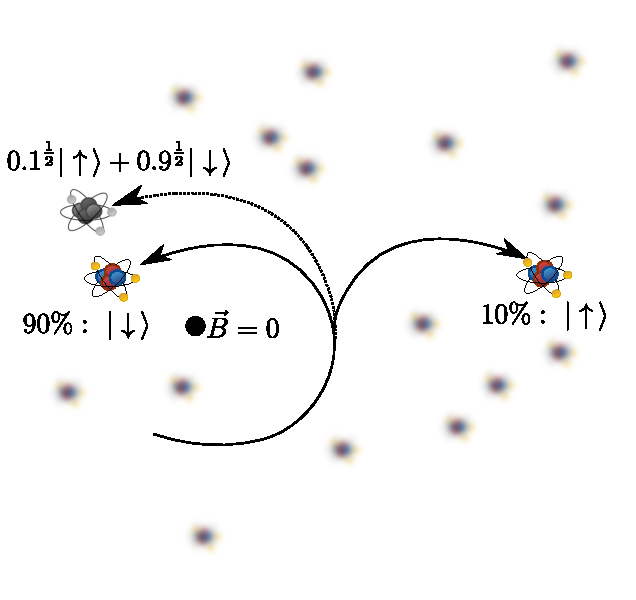
\includegraphics[width=0.75\textwidth]{figures/hidden_variables/evap_problem.pdf}
    \caption{todo}
    \label{fig:evap_problem}
\end{figure}

So how can we modify a semiclassical method to choose only one trajectory? Firstly, since each trajectory corresponds to one of the internal states (though some might be degenerate), our model must choose an internal state and use the classical trajectory corresponding to that internal state only. Secondly, since all atoms begin in identical states and yet some take one trajectory and some another, this choice must be probabilistic. Finally, the probabilities must be consistent with those from quantum mechanics, i.e. the Born rule: the probability of an atom taking each trajectory must be proportional to the squared amplitude of the internal state of the atom, projected onto the eigenstate corresponding to that trajectory.

There exists a category of theories dealing with precisely this question of how to choose a specific state of a quantum system in a stochastic way, such that the probability of having chosen a state is equal to that given by quantum mechanics. Such theories are called ``hidden variable'' theories, and the number specifying which state has been chosen is the ``hidden variable''.

\section{Hidden variable theories}

In his paper \emph{Quantum computing and dynamical quantum mdels}, Aaronson defines a ``dynamical quantum model''[CITE]:

\begin{quote}
A \emph{dynamical quantum model} assigns an eigenstate to a specified observable even when no measurement is made, and gives a stochastic evolution rule for that eigenstate. Such a model yields a distribution of classical histories of a quantum state
\end{quote}
In a later paper, \emph{Quantum computing and hidden variables}, superseding the first, Aaronson renames dynamical quantum models \emph{hidden-variable theories} and instead defines:
\begin{quote}
For us, a hidden-variable theory is simply a way to convert a unitary matrix that maps one quantum state to another, into a stochastic matrix that maps the initial probability distribution to the final one in some fixed basis
\end{quote}
This is what a hidden-variable theory is for the purposes of this chapter as well. Though the second paper supersedes the first, the definition it gives is more tangible for us---we wish to \emph{assign an eigenstate} to our atoms (choose one of the internal states in order to decide which trajectory to follow), and have a \emph{stochastic evolution rule} for which eigenstate is chosen at any one time (allow the atom to begin taking a different trajectory if it makes transitions between states).

But the second definition is more specific. The stochastic evolution rule is in the form of a stochastic matrix, with elements equal to transition probabilities for some time interval. And the rule should be in some way based on the unitary evolution that the quantum system evolves according to in the same interval of time, such that the initial and final probabilities of the stochastic matrix and unitary evolution agree. That is, if a quantum state $\ket\chi$ evolves in a certain basis $\{\ket{n}\}$according to a unitary $\hat U(t^\prime, t)$:
\begin{align}
\left[\begin{matrix}
\chi_1(t^\prime)\\\chi_2(t^\prime)\\\chi_3(t^\prime)\\\vdots
\end{matrix}\right]
= \left[\begin{matrix}
U_{11}(t^\prime, t) & U_{12}(t^\prime, t) & U_{13}(t^\prime, t)&\hdots\\
U_{21}(t^\prime, t) & U_{22}(t^\prime, t) & U_{23}(t^\prime, t)&\hdots\\
U_{31}(t^\prime, t) & U_{32}(t^\prime, t) & U_{33}(t^\prime, t)&\hdots\\
\vdots & \vdots & \vdots & \ddots
\end{matrix}\right]
\left[\begin{matrix}
\chi_1(t)\\\chi_2(t)\\\chi_3(t)\\\vdots
\end{matrix}\right],
\end{align}
where $\chi_n = \braket{n}{\chi}$ and $U_{nm}(t^\prime, t) = \matrixel{n}{\hat U(t^\prime, t)}{m}$, then a hidden variable theory is a matrix-valued function $S(U(t^\prime, t), \vec\chi(t)))$, where $\vec\chi(t)$ and $U(t^\prime, t)$ are the vector and matrix representations of the state vector $\ket\chi(t)$ and unitary $\hat U(t^\prime, t)$in the $\{\ket{n}\}$ basis, that satisfies:
\begin{align}
\left[\begin{matrix}
\abs{\chi_1(t^\prime)}^2\\\abs{\chi_2(t^\prime)}^2\\\abs{\chi_3(t^\prime)}^2\\\vdots
\end{matrix}\right]
= \left[\begin{matrix}
S_{11}(t^\prime, t) & S_{12}(t^\prime, t) & S_{13}(t^\prime, t)&\hdots\\
S_{21}(t^\prime, t) & S_{22}(t^\prime, t) & S_{23}(t^\prime, t)&\hdots\\
S_{31}(t^\prime, t) & S_{32}(t^\prime, t) & S_{33}(t^\prime, t)&\hdots\\
\vdots & \vdots & \vdots & \ddots
\end{matrix}\right]
\left[\begin{matrix}
\abs{\chi_1(t)}^2\\\abs{\chi_2(t)}^2\\\abs{\chi_2(t)}^2\\\vdots
\end{matrix}\right],
\end{align}
In essence, if quantum unitary evolution takes amplitudes to amplitudes, a hidden variable theory takes probabilities to probabilities. Thus the elements of $S$ are conditional probabilities---or transition probabilities---for a hidden variable $\eta(t)$, giving the chance that the state $\ket\eta \in \{\ket{n}\}$ assigned by the hidden variable will change from one to another in the given time interval:
[double check indices]
\begin{align}\label{eq:conditional_probability}
\Pr(\eta(t^\prime){=}i|\eta(t){=}j) = S(U(t^\prime, t), \vec\chi(t))_{ij}.
\end{align}

There are many ways to define functions $S$ that satisfy this condition. The simplest is to ignore the unitary completely and set $S_{ij} = \abs{\chi_i(t^\prime)}^2$ for all $n$, which yields:
\begin{align}
\Pr(\eta(t^\prime){=}i|\eta(t){=}j) = \abs{\chi_{i}(t^\prime)}^2,
\end{align}
that is that the hidden variable $\eta$ is equally likely to transition to a given value regardless of its previous value, and regardless of the unitary, and that that the conditional transition probability from all input states is just the squared amplitude of the final state. This theory represents a hidden variable that will just jump between states randomly based on their amplitude, with no regard for whether there were actually amplitude flows between the states between which it is transitioning. Nonetheless, it matches the definition of a hidden variable theory---$S$ is a stochastic matrix, and the hidden variable on average will spend an amount of time in each state consistent with the Born rule.

Aaronson outlines [CITE] some additional axioms that hidden variables ought to satisfy, if we are to take them seriously, including reasonable statements about symmetries, and insensitivity to small perturbations. He goes on to prove that the properties cannot all be satisfied simultaneously, but some theories satisfy more of them than others.

It is convenient to introduce the matrix $P$ of absolute transition probabilities. Summing \eqref{eq:conditional_probability} over all possible initial values of the hidden variable yields the absolute probability of it having a particular final value after the given time interval:
\begin{align}
\Pr(\eta(t^\prime){=}i) 
= \sum_j \Pr(\eta(t^\prime){=}i|\eta(t){=}j) \Pr(\eta(t){=}j),
\end{align}
which, recognising that the final and initial probabilities must be the final and initial squared amplitudes of the state vector, can be rewritten:
\begin{align}
\abs{\chi_i(t^\prime)}^2
= \sum_j S(U(t^\prime, t), \vec\chi(t))_{ij} \abs{\chi_j(t)}^2.
\end{align}
We now define the matrix of absolute transition probabilities $P$:
\begin{align}\label{eq:P_matrix_def}
P_{ij} = S_{ij}(U(t^\prime, t), \vec\chi(t)) \abs{\chi_j(t)}^2,
\end{align}
such that:
\begin{align}
\abs{\chi_i(t^\prime)}^2
= \sum_j P_{ij}.
\end{align}
So we have that $P$ has row sums equal to the final squared amplitudes.
And, because $P_{ij} = S_{ij}\abs{\chi_j(t)}^2$ and $S$ is a stochastic matrix with column sums equal to one,\footnote{In order to more clearly compare to quantum evolution, we are using \emph{left stochastic} matrices, which multiply column vectors of probabilities from the left, contrary to the most common convention for stochastic matrices which is to multiply row matrices from the right. Thus $S$ has unit column sums, whereas the corresponding right stochastic matrix (its transpose) would have unit row sums.} we have that $P$ must have row sums equal to the initial squared amplitudes.

Now that we have introduced $P$ and shown what its row and column sums must be, we come to a particularly simply defined hidden variable theory called the Schr\"odinger theory, discussed in Aaronson's hidden-variables paper [CITE]. The idea is to form $P$ by staring with the matrix of absolule values of $U$, and simply scaling its rows and columns to have the correct values:\footnote{One might expect that the absolute value squared might be a better choice, since this matches Fermi's golden rule. Aaronson argues in his paper, when discussing his own hidden-variable theory \emph{Flow theory} why absolute values of elements of the unitary have nice properties, and we show later that the row and column scalings reproduce Fermi's golden rule in any case, as they must for the hidden varaible theory to agree with quantum probabilities.}
\begin{align}
P = \left[\begin{matrix}
a_1b_1\abs{U_{11}(t^\prime, t)} & a_1b_2\abs{U_{12}(t^\prime, t)} & a_1b_3\abs{U_{13}(t^\prime, t)}&\hdots\\
a_2b_1\abs{U_{21}(t^\prime, t)} & a_2b_2\abs{U_{22}(t^\prime, t)} & a_2b_3\abs{U_{23}(t^\prime, t)}&\hdots\\
a_3b_1\abs{U_{31}(t^\prime, t)} & a_3b_2\abs{U_{32}(t^\prime, t)} & a_3b_3\abs{U_{33}(t^\prime, t)}&\hdots\\
\vdots & \vdots & \vdots & \ddots
\end{matrix}\right],
\end{align}
that is,
\begin{align}
P_{ij} = a_i b_j \abs{U_{ij}(t^\prime, t)},
\end{align}
where the row scalings $\{a_i\}$ and column scalings $\{b_j\}$ satisfy:
\begin{align}
\sum_j a_i b_j \abs{U_{ij}(t^\prime, t)} = \abs{\chi_i(t^\prime)}^2,\label{eq:a_scalings}\\
\sum_i a_i b_j \abs{U_{ij}(t^\prime, t)} = \abs{\chi_j(t)}^2\label{eq:b_scalings},
\end{align}
which can be solved numerically, and then the Schrodinger theory stochastic matrix then able to be extracted by inverting \eqref{eq:P_matrix_def}:
\begin{align}
S_{ij}(U(t^\prime, t), \vec\chi(t))
= a_i b_j \frac{\abs{U_{ij}(t^\prime, t)}}{\abs{\chi_j(t)}^2}.
\end{align}

\subsection{Numerically evaluating Schr\"odinger theory}

There are many ways to solve numerically for the row and column scalings, but there is one unique solution for the resulting scaled matrix.\footnote{The values of $\{a_i\}$ and $\{b_j\}$ are only determined up to an overall multiplication of each $\{a_i\}$ by a constant and division of each $\{b_j\}$ by the same constant, since only products $a_i b_j$ appear in the resulting scaled matrix} The simplest method is to simply alternate between scaling the rows to get the right row sums, then scaling the columns to get the right column sums, and repeating, that is, alternating between solving equation~\eqref{eq:a_scalings} for all $a_i$, and solving~\eqref{eq:b_scalings} for all $b_i$, until the result converges. This is called the Sinkhorn-Knopp method of r-c (row-column) scaling [CITE], but is computationally intensive, with slow convergence [CITE LINEAL]. An alternative is the method by Lineal et al [CITE], which converges much faster. Both are iterative methods, and so in practice one can save the resulting row and column scalings at each integration step of a simulation and use them as the initial guesses for the same computation at the next integration step,\footnote{With the caveat that since (as mentioned in the previous footnote) the row and column scalings are only determined up to an overall multiplication/division, occasional multiplication of all $\{a_i\}$ and division of all $\{b_i\}$ by a constant may be neccesary to prevent the values numerically overflowing or underflowing in the middle of a simulation.} providing considerable speedup.

For the case of a $2\times2$ system, the row and column scalings can be found analytically, with the result
\begin{align}
a_1 &= 1\\
a_2 &: a_2^2 + 
\left(\frac1{AB} - \frac AB \abs{\chi_1(t)}^2 - \frac BA \abs{\chi_2(t)}^2\right)a_2
+ \frac{\abs{\chi_2(t^\prime)}^2}{\abs{\chi_1(t^\prime)}^2} = 0\\
b_1 &= \frac{\abs{\chi_1(t^\prime)}^2}{A + B a_2}\\
b_2 &= \frac{\abs{\chi_2(t^\prime)}^2}{B + A a_2},
\end{align}
where $a_2$ is the positive solution to the given quadratic, $A = \abs{U_{11}} = \abs{U_{22}}$ and $B = \abs{U_{12}} = \abs{U_{21}}$. This result only holds in the case of Schr\"odinger theory for a state vector with two components subject to unitary evolution---not for row-column scaling in general---since it makes use of symmetries of unitary matrices and the fact that the initial and final probabilities given by the squared amplitudes of the state vector components must sum to unity.

A final note on numerics: the above expressions for Schr\"odinger theory and its analytic expression for a $2\times2$ system involve dividing by elements of the unitary, and state populations, both of which may be zero. Whilst the relevant limits may exist, we cannot easily compute them numerically, and so I have taken to simply replacing small values of $\abs{U_{ij}}$, $\abs{\chi_i(t^\prime)}^2$ and $\abs{\chi_j(t)}^2$ with a small constant  $\varepsilon=1\times 10^{-10}$, ensuring that the convergence criterion I pass to Lineal's method is larger 
 
TODO:
\begin{itemize}
\item Define/describe what a hidden variable theory is, drawing heavily on Aaronson's~\cite{Aaronson2005} explanations. Give examples, argue why the Schr\"odinger theory is appealing.

\item Motivate with Stern-Gerlach experiment, and derive the method, show what sorts of problems it
solves and where it disagrees with other models, provide simulation results. Limitations: no time dependent potentials, no 3D.

\item Possibly include speculation about these:

\item Maybe include a test to see whether it actually does work in 3D as-is, since we haven't actually checked, we just haven't been able to show on paper that current behavior is correct in 3D (also haven't shown it's incorrect).

\item Time dependent potentials could potentially be handled by approximating unitary as product of part due to spatial variation in H, and part due to time variation in H. compute transition probs for both such that a transition can be attributed to one or the other - only do velocity jumps to conserve potential if due to spatial motion, as time dependent potential can exchange energy with particle.

\item Matrix scaling for Schrodinger theory, discuss methods: Sinkhorn-Knopp, Lineal, and my one. Compare time complexity of algorithms so as to define the computational complexity of the hidden variables semiclassical method. Method is of course parallelisable on GPU or similar so is fast on parallel machines even if matrix scaling is slow.

\item Discuss how it would make sense for the systems to behave in the presence of collisions w.r.t collapse of state vectors.

\item Be sure to include picture from KOALA talk of atoms going in multiple directions
\end{itemize}

\section{Approximate Markovian decoherence rate for separating wavepackets}

Positional separation of two different internal states of an atom leads to decoherence of those states, with a decoherence factor $r_{ij}(t)$ equal to the overlap of the spatial wavefunctions of the two components in question a time $t$ after they began separating. Approximating both wavepackets as initially overlapping Gaussians of width $\sigma$, ignoring dispersion, and assuming they separate with constant relative acceleration $a_{ij}$, the decoherence factor is

\begin{align}
r_{ij}(t) &= \braket{\psi_i(t)}{\psi_j(t)}\\
 &= C \int_{-\infty}^{\infty} e^{-\frac{x^2}{4\sigma^2}}e^{-\frac{(x-x_\up{rel})^2}{4\sigma^2} + ik_\up{rel}x}\,\dd x,\label{eq:gaussian_integral}
\end{align}
where
\begin{align}
x_{\mathrm{rel}}(t) = \frac12a_{ij}t^2
\end{align}
and
\begin{align}
k_\up{rel}(t) = \frac m \hbar a_{ij} t
\end{align}
are the wavepackets' relative\footnote{$a_{ij}$, $x_\up{rel}$ and $k_\up{rel}$ are the acceleration, position, and wavenumber of the $j^\up{th}$ component with respect to the $i^\up{th}$ component, that is, $a_{ij} = a_j - a_i$, etc.} position and wavenumber due to acceleration for a time $t$ starting from zero relative velocity, and
\begin{align}
C^{-1}=\int_{-\infty}^\infty e^{-\frac{x^2}{2\sigma^2}}\,\dd x\label{supp:eq:Cdef}
\end{align}
is a normalisation constant [TODO CHECK IF NEEDS TO BE SQUARED]. Note that this expression holds for any number of dimensions---relative motion is only along one axis so the integrals in all other directions equal one.

Evaluating the Gaussian integral \eqref{eq:gaussian_integral} gives the following expression for the decoherence factor $r_{ij}(t)$:
\begin{align}
r_{ij}(t)&= e^{-\left[
        \frac{1} {8\sigma^2} x_\up{rel}^2
      + \frac i2 x_{\mathrm{rel}} k_\up{rel}
      + \frac{\sigma^2}{2} k_\up{rel}^2
      \right]}\label{eq:decoherence_factor}.
\end{align}

This is a decoherence \emph{factor}; it is the factor by which the $(i, j)$ off-diagonal of the reduced density matrix for the atom's internal state will be reduced at time $t$. The corresponding decoherence \emph{rate} is given by the logarithmic derivative of \eqref{eq:decoherence_factor}:

\begin{align}
\Gamma_{ij}(t) = - \frac 1 {r_{ij}(t)} \dv t {r_{ij}(t)}.
\end{align}

 The fact that \eqref{eq:decoherence_factor} does not describe a constant decoherence rate (i.e., it does not have the functional form of exponential decay) means that the back-action on the atom's internal state caused by measurements of its motional state will be different depending on the interval of time between measurements.

For example, the logarithmic derivative of \eqref{eq:decoherence_factor} approaches zero as $t$ goes to zero. This means that in the limit of infinitely frequent measurements, no decoherence occurs at all in between measurements, and the motional state is reset after each measurement such that the wavepackets never separate at all. This is the quantum Zeno effect, and its appearance in models of open quantum systems is usually treated as a reminder that the assumption of infinitely frequent strong measurements is unphysical [CITE].

Since experimentally we are not measuring atoms' motional states so frequently, we ought to wait until the wavepackets are completely separated before performing a projective measurement. As in quantum optics models of open quantum systems, in which the measurement interval ``should be large enough to allow the photons to get away from the atom" [CITE The Quantum Jump Approach
and Quantum Trajectories Gerhard C. Hegerfeldt], ours should be large enough for the atomic states to get away from each other.

If at large enough times, a decoherence rate is independent of time, that decoherence is called Markovian at that timescale. A Markovian environment is one that has no memory of the decoherence process---it ``forgets" any information caused by past interaction with the system. Even though at short times, all decoherence rates in quantum mechanics tend to zero [CITE], if they become Markovian on a timescale shorter than other timescales of interest, the Markov approximation can be used and a constant decoherence rate used at all times. In quantum optics, the decoherence factor for the internal state of an atom due to photon emission indeed tends to exponential decay on timescales that are still much shorter than that of the system evolution, and thus the Markov approximation is accurate.

Unlike quantum optics models, our decoherence factor does not describe Markovian decoherence on any timescale. In the limit of large $t$, its functional form is $e^{-t^4}$, not the exponential decay required to treat the decoherence as Markovian [CITE] at that timescale. Nonetheless, if we wish to write a time-local differential equation for the internal state of the atom, Markovian decoherence is the only kind we can include [CITE].

To that end, we will now construct a ``time ignorant" version of $r_{ij}(t)$ that answers the question ``What is the expected decoherence factor at all future times, if you don't know how long it has been since the two wavepackets began separating?" In this way we can compute an \emph{average} decoherence rate $\Gamma_{ij}$ described by our decoherence factor, even though $r_{ij}(t)$ does not have a constant decoherence rate at large times. This essentially amounts to finding the best fitting exponential to $r_{ij}(t)$. Whilst this approximation is crude, it is nonetheless an improvement over the Ehrenfest model, which has no decoherence at all (i.e. it has a decoherence rate that is also constant like ours---but equal to zero).

\begin{figure}[t]
    \centerfloat
    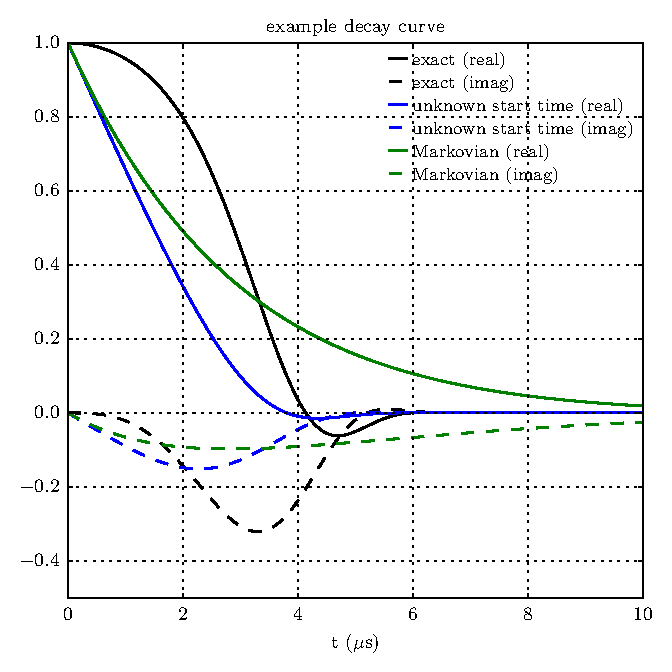
\includegraphics{figures/hidden_variables/decoherence_factor_example.pdf}
    \caption{Caption.}
    \label{fig:decoherence_factor_example}
\end{figure}

We define the time-ignorant decoherence factor $\tilde r_{ij}(t)$ as the overlap of the wavefunction of the $i^\up{th}$ internal state with a superposition of wavepackets of the $j^\up{th}$ internal state, with the superposition being over all times in the past the wavepackets began separating:
\begin{align}
\tilde r_{ij}(t) &= \bra{\psi_i(t)} A\int_{-\infty}^0 \ket{\psi_j(t - t^\prime)} \,\dd t^\prime,
\end{align}
where $A$ is a normalisation constant such that $\tilde r_{ij}(0) = 1$.
Since $\ket{\psi_i(t)}$ is time independent (rather, since we can perform our calculations in the frame of reference in which it is stationary), this is:
\begin{align}
\tilde r_{ij}(t) &= A\int_{-\infty}^0 r_{ij}(t - t^\prime) \,\dd t^\prime,
\end{align}
which is simply the convolution of our decoherence factor with a step function which is nonzero at all negative times.
Our average decoherence rate $\Gamma_{ij}$ is then given by the logarithmic derivative of $\tilde r_{ij}(t)$ at $t=0$:

\begin{align}
\Gamma_{ij} &= -\frac {\tilde r_{ij}^\prime(0)} {\tilde r_{ij}(0)}\\
&= -\frac {\int_0^\infty \tilde r_{ij}^\prime(t)\,\dd t} {\int_0^\infty \tilde r_{ij}(t)\, \dd t}\\
\Rightarrow \Gamma_{ij}^{-1}&= \int_0^\infty e^{-\left[
        \frac{1} {8\sigma^2} x_\up{rel}^2
      + \frac i2 x_{\mathrm{rel}} k_\up{rel}
      + \frac{\sigma^2}{2} k_\up{rel}^2
      \right]}\, \dd t.\label{eq:gamma_integral}
\end{align}

As mentioned, $\Gamma_{ij}$ is the decay constant for the best fitting exponential to our decoherence factor \eqref{eq:decoherence_factor}. Although \eqref{eq:decoherence_factor} looks nothing like a decaying exponential in time, an exponential approximation to it nonetheless ought to decay to zero on the same timescale. An example of this is shown in \figref{fig:decoherence_factor_example}

In order to obtain an approximate analytic expression for this integral, we consider two limiting cases and then stitch them together in the intermediate regime. In the limit of small wavepackets, $\sigma$ is small and thus the first term in the exponent in \eqref{eq:gamma_integral} is largest, and the third term is smallest. In this regime, which describes when positional separation (as opposed to separation in $k$-space) dominates the decoherence, we'll neglect the third term in the exponent and treat the second term as small relative to the first.
This gives us:
\begin{align}
\Gamma_{ij\,\up{(pos)}}^{-1} &\approx \int_0^\infty e^{-\left[
        \frac{1} {8\sigma^2} x_\up{rel}^2
      + \frac i2 x_{\mathrm{rel}} k_\up{rel}
      \right]}\, \dd t.\\
      &\approx \int_0^\infty e^{-
              \frac{1} {8\sigma^2} x_\up{rel}^2}\left(1 - \frac i2 x_{\mathrm{rel}} k_\up{rel}\right)\, \dd t.\label{eq:gamma_pos_exp}\\
      &= 2^{\frac54}\upGamma(\tfrac54)\sqrt{\frac{\sigma}{a_{ij}}} - 2i\frac{m \sigma^2}{\hbar},\label{eq:gamma_pos_recip}
\end{align}
where we used a first-order Taylor expansion of an exponential in \eqref{eq:gamma_pos_exp}. We similarly use a first order expansion to take the reciprocal of \eqref{eq:gamma_pos_recip} (since the second term is much smaller than the first\footnote{This isn't necessary in order to obtain a simple expression for $\Gamma_{ij\,\up{(pos)}}$---the reciprocal without this approximation is equally simple---but it leaves us with power laws for the real and imaginary parts of $\Gamma_{ij\,\up{(pos)}}$, which are easier to stitch together with those from the large $\sigma$ regime.}), and arrive at:
\begin{align}
\Gamma_{ij\,\up{(pos)}} &\approx \frac1{2^{\frac54}\upGamma(\tfrac54)}\sqrt{\frac{a_{ij}}{\sigma}}
+ \frac i {2\sqrt{2}\upGamma(\tfrac54)^2} \frac{m\sigma a_{ij}}{\hbar}\label{eq:gamma_pos_final}%\\
% &\approx 0.463865\sqrt{\frac{a_{ij}}{\sigma}}
% + 0.430341 i \frac{m\sigma a_{ij}}{\hbar}.
\end{align}

Similarly for the large $\sigma$ regime, we neglect the first term in the exponent of \eqref{eq:gamma_integral} and consider the second term small relative to the third. This is the regime in which the decrease in overlap of the two wavepackets is dominated by their separation in velocity space. Following the same process as above gives:
\begin{align}
\Gamma_{ij\,\up{(vel)}}^{-1} &\approx \int_0^\infty e^{-\left[
        \frac i2 x_{\mathrm{rel}} k_\up{rel}
        + \frac{\sigma^2}{2} k_\up{rel}^2
      \right]}\, \dd t.\\
      &\approx \int_0^\infty \left(1 - \frac i2 x_{\mathrm{rel}} k_\up{rel}\right)
      e^{-\frac{\sigma^2}{2} k_\up{rel}^2}\, \dd t\\
      & = \sqrt{\frac\pi2}\frac\hbar{m \sigma a_{ij}} - i\frac{\hbar^3}{2m^3 \sigma^4 a_{ij}^2}\\
      \Rightarrow \Gamma_{ij\,\up{(vel)}} &\approx \sqrt{\frac2\pi}\frac{m \sigma a_{ij}}\hbar
                                          + \frac i\pi \frac\hbar{m \sigma^2}
                                          \label{eq:gamma_vel_final}
\end{align}
Equations \eqref{eq:gamma_pos_final} and \eqref{eq:gamma_vel_final} are our final expressions for the docoherence rate in the limit of small and large wavepackets respectively. Adding their real parts in quadrature and adding the reciprocals of their imaginary parts then provides a reasonable approximation for $\Gamma_{ij}$ over all wavepacket sizes:
\begin{align}
\Gamma_{ij} \approx
\left[\re(\Gamma_{ij\,\up{(pos)}})^2 + \re(\Gamma_{ij\,\up{(vel)}})^2\right]^{\frac12}
+ i\left[\im(\Gamma_{ij\,\up{(pos)}})^{-1} + \im(\Gamma_{ij\,\up{(vel)}})^{-1}\right]^{-1}.
\label{eq:gamma_total}
\end{align}

\begin{figure}[t]
    \centerfloat
    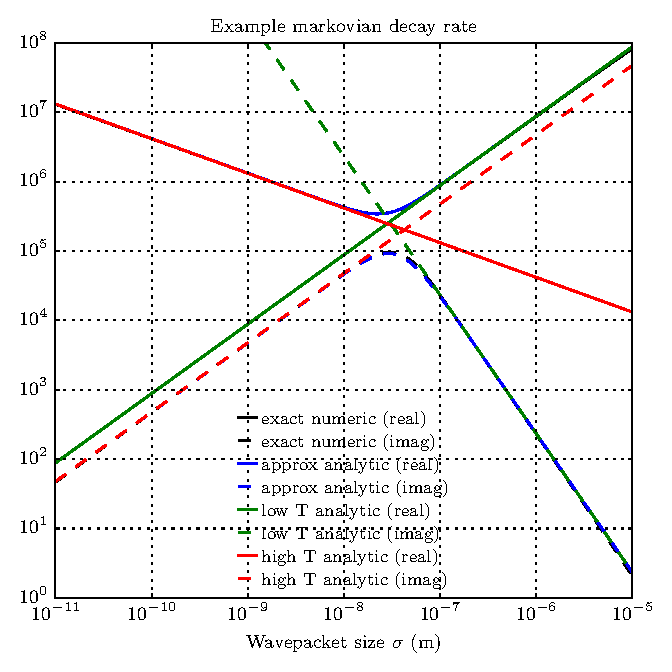
\includegraphics{figures/hidden_variables/decoherence_rate_example.pdf}
    \caption{Caption.}\label{fig:decoherence_rate_example}
\end{figure}

We now have an approximate analytic expression that is computationally inexpensive to evaluate for each atom in an ensemble at every timestep of a differential equation.
An example showing the accuracy of \eqref{eq:gamma_total}, compared to the exact expression \eqref{eq:gamma_integral} for $\Gamma_{ij}$ over a range of wavepacket sizes is shown in \figref{fig:decoherence_rate_example}.

\section{Choice of wavepacket size}

How big is a wavepacket?
